\documentclass[doublecol,linenumbers]{epl2} % for 2 columns style with line numbers
% or \documentclass[doublecol]{epl2} for 2 columns style without line numbers
% or \documentclass[page-classic,linenumbers]{epl2} for one column style with line numbers
% or \documentclass[page-classic]{epl2} for one column style without line numbers

\usepackage{textcomp}
\usepackage{multirow}
%\usepackage{todonotes}
%\usepackage[colorinlistoftodos]{todonotes}
\usepackage[inline]{trackchanges}

\addeditor{kate}
\addeditor{mikhail}
\addeditor{egor}

\title{Estimation of number of runaway electrons per avalanche in Earth's atmosphere}
\shorttitle{Number of runaway electrons per avalanche  in Earth's atmosphere} %Insert here a short version of the title if it exceeds 70 characters

\author{
T. Khamitov\inst{1,2}\thanks{E-mail: \email{timuruh@mail.ru}} 
\and 
A. Nozik\inst{1,2}\thanks{E-mail: \email{nozik.aa@mipt.ru}} \and 
E. Stadnichuk\inst{1,2}\thanks{E-mail: \email{egrstadnichuk@yandex.ru}} \and 
E. Svechnikova\inst{3}\thanks{E-mail: \email{svechnikova@ipfran.ru}}  \and
M. Zelenyi\inst{1,2}\thanks{E-mail: \email{mihail.zelenyy@phystech.edu}}
 %\and M. Dolgonosov\inst{3, 5}\thanks{E-mail: \email{cactus@iki.rssi.ru}}
}

\shortauthor{M. Zelenyi \etal}

\institute{                 
  \inst{1} Moscow Institute of Physics and Technology (National Research University) - 1 “А” Kerchenskaya st., Moscow, 117303, Russian Federation \\
  \inst{2} Institute for Nuclear Research of RAS - prospekt 60-letiya Oktyabrya 7a, Moscow 117312\\
  %\inst{3} Space Research Institute of RAS - 84/32 Profsoyuznaya str., 117997, Moscow, Russia\\
  \inst{3} Institute of Applied Physics of RAS - 46 Ul'yanov str., 603950, Nizhny Novgorod, Russia
%   \\
%   \inst{5} National Research University Higher School of Economics - 20 Myasnitskaya str., 101000, Moscow, Russia
}
% \pacs{nn.mm.xx}{First pacs description}
% \pacs{nn.mm.xx}{Second pacs description}
% \pacs{nn.mm.xx}{Third pacs description}

\begin{document}
\abstract{
    The connection between thunderstorms and relativistic runaway electron avalanches is an important topic that has attracted the attention of many researchers. Among other things, there are a lot of various simulations of the dynamics of electron avalanches. This article was written mostly in response to article "The critical avalanche of runaway electrons" by Evgeny Oreshkin, which shows rather large numbers for estimate of number of runway electrons, but it also contains the results of our own simulation and comparison with other papers.
}

\maketitle

\section{Introduction}
The phenomenon of relativistic runaway electron avalanche (RREA) development in atmospheric electric field is the generally accepted mechanism for enhancement of low energy gamma~(10~keV~--~100~MeV) and electron fluxes in Earth's atmosphere \cite{Dwyer2014,CHILINGARIAN201468}. This mechanism draws additional attention because it could bring the light to the problem of lightning discharge generation which up to this point does not have a satisfactory explanation. Additionally, there is a number of observed phenomena (like Terrestrial Gamma-Ray Flashes~(TGFs) \cite{Dwyer2012} and Thunderstorm Ground Enhancements~(TGE) \cite{CHILINGARIAN201468}) believed to be have an origin related to RREA. However, the certain conditions of the formation of avalanches and dynamics of its development remain unknown. There are several articles presenting an analytical model of avalanche development. For example, \cite{gurevich1992runaway, Babich2001, Dwyer2007, lehtinen1999monte}.
%\change[mikhail]{There are a number of articles presenting an analytical model of avalanche development, the most \change[kate]{outstanding}{advanced} of which is \cite{Gurevich:2001}.}{a}
%\todo[inline]{"However, the certain conditions of the formation of avalanches and dynamics of its development remain unknown." - what do we mean by this statement?}
Numerical modeling of energetic particle propagation in air leading to an avalanche generation is presented in another set of papers \cite{moss2006, DwyerSmith2005, skeltved2014}.

A recent paper \cite{Oreshkin_2018} presents the results of 3D Monte-Carlo simulation of runaway avalanche development. The paper is focused on the avalanche-to-streamer transition. One of the main results is the estimation of the number of electrons in one avalanche: $10^{17}$ - $10^{18}$. The value is significantly larger, than values presented in other simulations (\cite{Gurevich:2001, dwyer2003fundamental,dwyer2011low}), which show about $10^6$ fast electrons and $10^{10}$ slow electrons per in avalanche in normal conditions (air pressure, gas composition etc.). The difference could be attributed to some non-standard approximations made in the article.

In our article we put those results to test using some rough (upper bound) analytical estimation as well as simulation results of RREA accomplished with software designed by our group on the basis of GEANT4 libraries.

\section{Analytical estimation of number of runaway electrons}

A simple analytical estimation of number of runaway electrons can be obtained on the basis of the theory of runaway breakdown~\cite{Gurevich:2001}. Lets consider acceleration and avalanche multiplication of electrons in uniform electric field. According to~\cite{Gurevich:2001} number of runaway electrons in a RREA grows exponentially with coordinate z:
\begin{equation}
\label{eq:exp}
    N(z) = N_0 \cdot e^{\frac{z}{l_a}}
\end{equation}
where $l_a$ --- characteristic length of generation of runaway electron, which can be estimated by the following formula:
\begin{equation}
    l_a = a\frac{2 m c^{2}}{e} \frac{1}{E}
\end{equation}
Here $m$ --- electron mass, $c$ --- speed of light, constant $a \approx 11$, $E$ --- electric field value. This model has in fact some limitations, since for higher electron energies (over 80~MeV), radiative losses start to dominate, but it produces correct upper estimate. 
%\todo[inline]{Could someone possibly be so kind to give here more details on limitations? What exactly limitations are? Mikhail: I think there is no need, this is a standard theory of ionization losses }
% \change[mikahil]{For a single primary runaway electron at the beginning of the region with electric field, number of runaway electrons at the end of the region of the strong field can be estimated in a following way:
% \begin{equation}
% \label{eq:num}
%     N(L) = e^{\frac{e E L}{2a m c^2 }}
% \end{equation}
% where $L$ is the length of the region with the strong electric field.  
% }
Alternatively, one can use empirical formula from Monte-Carlo simulation performed by Dwyer~\cite{Dwyer2007}:
\begin{equation}
\label{eq:dwyer}
    l_a = \frac{7300 kV}{E - 276 \frac{kV}{m} \cdot \frac{n}{n_0}},
\end{equation}
where $E$ is the value of the electric field, $n$ - air concentration and $n_0$ - air concentration under normal conditions. Using either of these formula, we can calculate the number of runaway electrons depending on size of the region with field and the field strength according to Eq.~\ref{eq:exp}. 
% It should be noted that Gurevich formula for multiplication length is derived within assumption that electric field is slightly higher than critical. In the simplified model multiplication length does not depend on the gas density.
% \change[kate]{. However, for the higher electric field strength values it should be taken into account.}{, which makes the model inapplicable for electric fields exceeding...~kV/m}
% \todo[inline]{How strong electric field needs to be in order to make the dependence important?}
Figure~\ref{fig:gur} shows the number of runaway electrons for different atmospheric conditions. For reasonable conditions  (region of vertical size 1200~m with electric field up to 200~kV/m) the number of runaway electrons does not exceed $10^{10}$.
\begin{figure}[h]
    \centering
    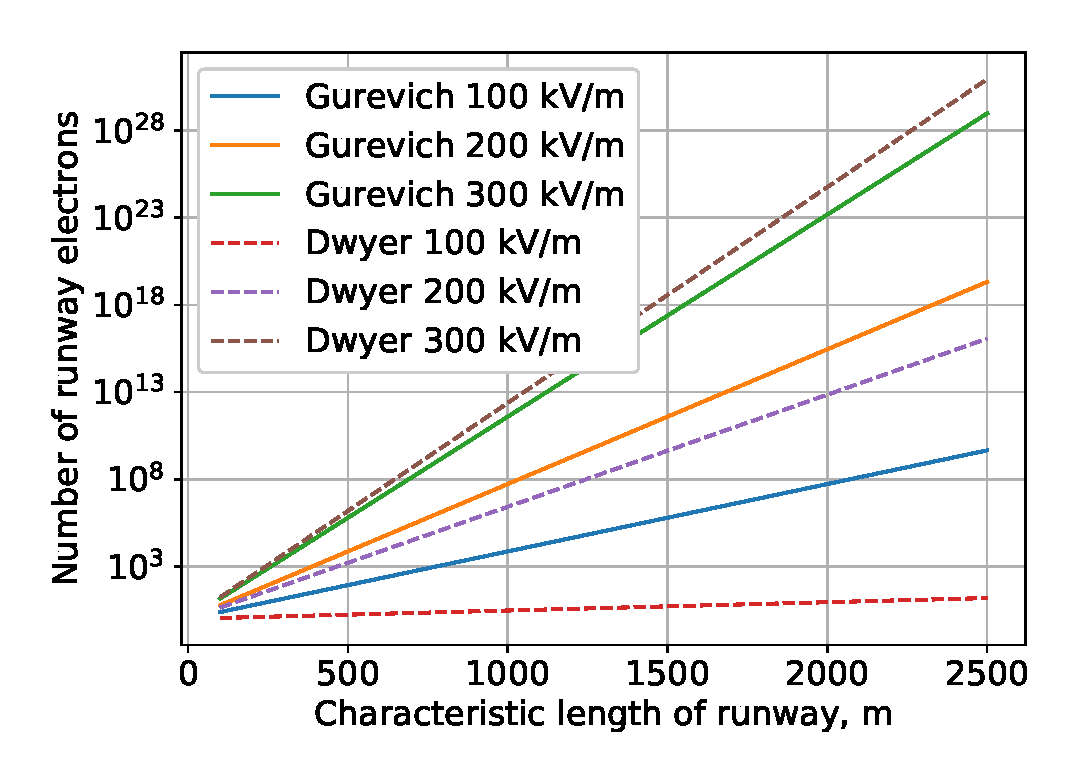
\includegraphics[width=0.45\textwidth]{figures/gurevich.eps}
    \caption{Number of runaway electrons in single avalanche in respect to avalanche length.}
    \label{fig:gur}
\end{figure}

\section{Simulation with GEANT4}
More accurate estimation of characteristic growth length of runaway electron avalanche could be obtained using GEANT4 transport code~\cite{Geant2003,Geant2006, Geant2016}, a standard tool for Monte-Carlo simulation in high energy physics (in this work we use version 4.10.05). The particle propagation mechanism used in GEANT4 is quite different from the one used in \cite{Oreshkin_2018}. GEANT4 uses particle tracks, meaning that each particle and its descendants. The simulation in \cite{Oreshkin_2018} uses particle population evolution in time. The evolutionary approach is useful for low-energy particle and plasma dynamics but usually is not used for precise simulation of high energy particles. GEANT4 allows to track gamma-rays and positrons as well as electrons, which is important for electron energies above 10~MeV. In order to investigate the role of processes involving positrons and gammas, we conducted three types simulations: 
\begin{enumerate}
    \item tracing electrons (and not considering any influence from gamma and positrons),
    \item tracing electrons and gammas, 
    \item electrons, gammas and positrons taken into account. 
\end{enumerate}

All our simulation use a lower energy threshold for particle generation of 0.05~MeV (particles born with lower energies are recorded, but nor propagated further).

Depending on the energy range, GEANT4 provides several models of physics processes, which are defined in physics lists. We use physics list \textit{G4EmStandardPhysics}, which takes into account following electrons interactions:

\begin{itemize}
    \item ionization loss,
    \item Coulomb scattering,
    \item multiple scattering,
    \item bremsstrahlung,
    \item gamma scattering and absorption,
    \item positron generation and annihilation.
\end{itemize}
It should be noted, that there is a physics list \textit{G4EmStandardPhysics\_opt4}. It contains the same physical processes, but uses advanced algorithm for tracking and requires much more processing time. Previous research shows that basic physics list gives higher estimate for the number of runaway electrons, so it could be used for upper boundary estimation~\cite{npmdwyer}.
In the simulation we use  vertical cylinder cloud geometry. The radius of the cylinder in this case is defined to be much larger than cylinder height so horizontal dimension is effectively infinite. The electric field is directed along the cylinder axis. An example of avalanche simulation without positron is shown on Fig.~\ref{fig:geant4}.
\begin{figure}[h]
    \centering
    \includegraphics[width=0.45\textwidth]{figures/geant4.eps}
    \caption{Example of GEANT4 simulation without positron: red tracks --- electrons, green tracks --- gamma-rays.}
    \label{fig:geant4}
\end{figure}
One of the main reasons behind simulation approach in \cite{Oreshkin_2018} is to limit otherwise very large simulation time and memory footprint. GEANT4 in general shares the same problem, but allows us to set an upper limit by calculating only multiplication length in Gurevich model. For longer acceleration volumes, the effective number of produced electrons is smaller than for small ones possibly because higher energy electrons tend to loose energy by producing high energy bremsstrahlung photons rather than secondary electrons. Photons also could produce electron avalanches, but those avalanches are in general separated from the main avalanche by hundreds of meters.

The simulation was carried out for following parameters of the system:
\begin{itemize}
    \item air density $0.4~kg/m^3$ (corresponds to atmospheric pressure $\sim 0.25~atm$ or the height 10~km for normal conditions);
    \item electric field --- $200~kV/m$ (the maximum electric field typically measured in thunderclouds~\cite{rakov_uman});
    \item acceleration cell height --- $800~m$ for simulation without positrons and $700~m$ for simulation with positrons (as we will see in result this length is approximately equal to 10 characteristic lengths and allows to accept the estimation as consistent).
\end{itemize}

In each case we inject 1000 initial electrons to the top of the cylinder (all results are  normalized by the number of initial electrons). Results of simulation are shown on Fig.~\ref{fig:sim}. Introduction of gamma does not significantly affect the results, so we do not present results with electrons only and with electron and gamma separately.

\begin{figure}[h]
    \centering
    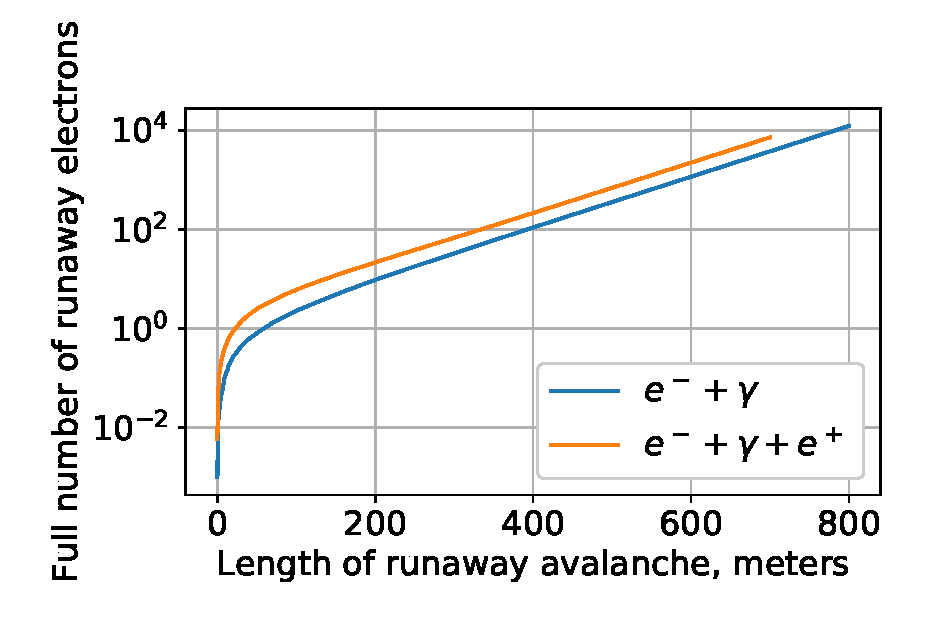
\includegraphics[width=0.45\textwidth]{figures/simulation.eps}
    \caption{Full number of runaway electron depending on the length of runaway avalanche: blue line --- simulation without positrons, orange line --- with positrons.}
    \label{fig:sim}
\end{figure}

The simulation data was fitted by exponential function from Eq.~\ref{eq:exp} with $N_0 = 1$ and $l_a$ as a free parameter. The resulting value is $l_a \approx 85 m$ without positron, and $l_a \approx 78~m$ with positrons. For comparison,~Eq.~\ref{eq:dwyer}~(Dwyer's formula) predicts $l_a \approx 64~m$). Using these values for characteristic length, we can estimate full number of runaway electrons in avalanches for different acceleration lengths. The results are presented in Table~\ref{tab:approx}. For reasonable acceleration cell lengths  $1200 - 1700$~meters it gives only $10^6-10^8$ runaway electrons, which is by many order less than $10^{16}$ predicted by \cite{Oreshkin_2018}. $10^{18} - 10^{19}$~runaway electrons could be obtained only for cell lengths closer to 4000 meters which are not possible in real atmospheric conditions.

\begin{table}[h]
    \centering
\begin{tabular}{crrr}
\hline
& & \multicolumn{2}{r}{Number of runaway electrons} \\
&   Length, m &   without positron &  with positron \\
\hline
\multirow{4}*{\rotatebox[origin=c]{90}{ simulation}} & 300 &  34.3      &  46 \\
& 500 &  361     &  589 \\
& 700 &  3802     &  7539 \\
& 800 &  12350 &  --- \\
\hline
\multirow{5}*{\rotatebox[origin=c]{90}{extrapolation}}& 1200 &  1.4e+06 &  4.3e+06 \\
& 1700 &  5.0e+08 &  2.5e+09 \\
& 2000 &  1.7e+10 &  1.2e+11 \\
& 4000 &  2.9e+20 &  1.3e+22 \\
& 5000 &  3.7e+25 &  4.5e+27 \\
\hline
\end{tabular}
    \caption{Estimate of the total number of runaway electrons based on 700-800 meter simulation. First part of table is taken from the simulation, second part is the extrapolation of simulation data.}
    \label{tab:approx}
\end{table}

When discussing lightning breakdown, it is important to compute not only number of breakdown electrons, but also total number of electrons and ions generated. This number could be very roughly estimated from energy conservation law. 

Number of ions produced by a single RREA can be estimated using the following logic. Firstly, all of energy runaway electrons receive from the electric field is spent on ionization, on production of new runaway electrons and on acceleration. Received energy in a segment $[z, z + dz]$ is approximately $N(z) e E d z$. Here $e$ is the electron electric charge, and all of runaway electrons are considered to move parallel to the $z$ axis. Further, the energy, spent on runaway electron production is about $\frac{d N(z)}{d z} \varepsilon_{0} d z$, where $\varepsilon_{0}$ is the mean kinetic energy of a runaway electron for conditions under consideration. Substitution of $\varepsilon_0$ in this formula also takes into consideration the acceleration of runaway electrons. According to Babich \cite{Babich2001}, the mean energy of RREA can be estimated as $\varepsilon_0 = e(E - E_c) l_a$, where $E_c$ is the critical electric field value. Consequently, in the frame of Dwyer's e-folding length the mean energy is simply derived as $\varepsilon_0 = 7.3~MeV$~\cite{Dwyer2007}. Finally, number of ions is calculated as the subtraction of received energy and energy wasted on runaway electron production, all divided by ionization potential. Ionization potential is considered to be 15~eV. Therefore, after integration the following estimation of number of ions is derived:
\begin{equation}
    N_{ions}(z) = \frac{e E l_a - \varepsilon_0}{I} \left( e^{\frac{z}{\l_a}} - 1\right).
\end{equation}

For $z = 1000~m$ we get $N_{ions} \approx 10^7$.
% \begin{equation}
%     N_{ion} = \frac{N_{runaway}*L*100 [keV/m] }{E_{ion}} \approx 10^{10}.
% \end{equation}

\section{Discussion}
Although he full Monte-Carlo simulation could not be carried out for a cell with vertical size more than 1000~m, the avalanche evolution on a larger scale could be characterised on the basis of extrapolation of the modeling results.
There is no physical mechanism that predicts a dramatic increase in the number of produced electrons for larger cells. On the contrary, as the length of the cell grows, the mean energy of runaway electrons grows as well until radiative losses start to dominate.
 %\todo[inline]{"On the contrary, as the length of the cell grows, grows the mean energy of runaway electrons." - it is a questionable statement. In fact, for small scale cells it's true. But on scales when $L >> \lambda_{RREA}$ the avalanche should become stable. Avalanche stability means that its spectrum remains the same.}
Electrons with higher energies tend to loose energy by emitting high-energy photons instead of direct production of additional electrons. The photons could produce secondary avalanches, but those avalanches have lower survival rates than the ones from secondary electrons and are in general separated from the main shower shaft. This fact is illustrated by simulation, presented at Fig.~\ref{fig:sec}. %\todo[inline]{I suppose that here we need some clarification about figure 4. It's not clear for me enough how we get from photon emission of high energy electrons to avalanche rates on small-scale 100 m cell. And, moreover, bremsstrahlung plays dominant role only with energies > 80 MeV in air, so we are in fact far from it.}
It shows the number of secondary electrons depending on initial electron energy. It could be seen that there is no significant yield change for initial energies above 5-10~MeV. Radiative loses prevent electrons from acquiring energies significantly higher than 60~MeV.

\begin{figure}[h]
    \centering
    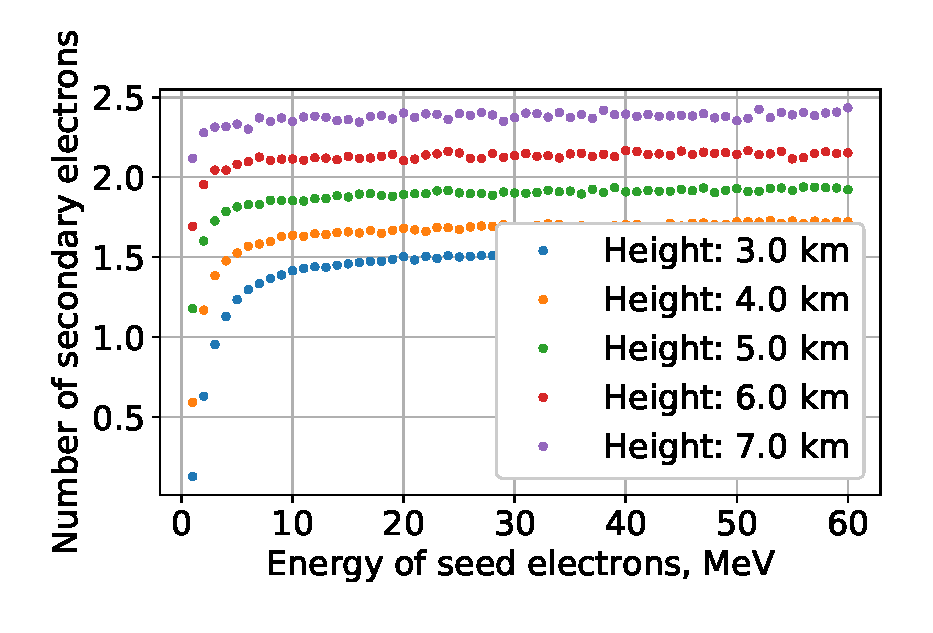
\includegraphics[width=0.45\textwidth]{figures/secondary.eps}
    \caption{The number of electrons escaping $100~m$ length volume depending on initial energy of the electron. Electric field --- $200~kV/m$. Figure shows that number of secondary particles does not depend on initial particle energy for energy over $10~MeV$}
    \label{fig:sec}
\end{figure} 

Dwyer positron feedback mechanism \cite{Dwyer2012feedback} could in theory produce significant increase in the number of runaway electrons, but recent research shows that the feedback value in this mechanism was rather overestimated~\cite{npmdwyer}.
%\todo[inline]{On our last seminar considering Dwyer's models we came to conclusion that Dwyer does not overestimate his feedback processes that significantly. For example, we estimated his feedback conditions for 0.4 density and 200 field. According to his graph, cell length ~ 600 m required for infinite feedback. According to our calculations it's ~700-800 m. Not that significant. So I wouldn't claim here something about feedback, let's make it more clear in our next article about Dwyer.}

In any case, both in this article and in \cite{Oreshkin_2018} we consider only forward avalanche motion without any feedback mechanisms. Still, our results show that it is not correct to completely ignore the positrons, which is even more significant for a cell with vertical size exceeding 1000 m. It happens mostly because positron production is the main interaction channel for high-energy photons. 
%\todo[inline]{How positron production could be the main mechanism if its length is in 2 orders larger than e.g. compton length on our energies? It's true for > 1 GeV energies. Or maybe we mean something else by these words?}

The radial distribution of runaway electrons production is demonstrated at Fig.~~\ref{fig:rad}. It could be seen that electrons have a wide horizontal distribution. This fact further reduces credibility of claims that those avalanches are the source of lightning breakdown, since the produced charge is distributed across rather large region. The horizontal spreading is significantly larger when  positrons taken into account because in this case photons could transfer the secondary avalanches far from initial ones.

\begin{figure}[h]
    \centering
    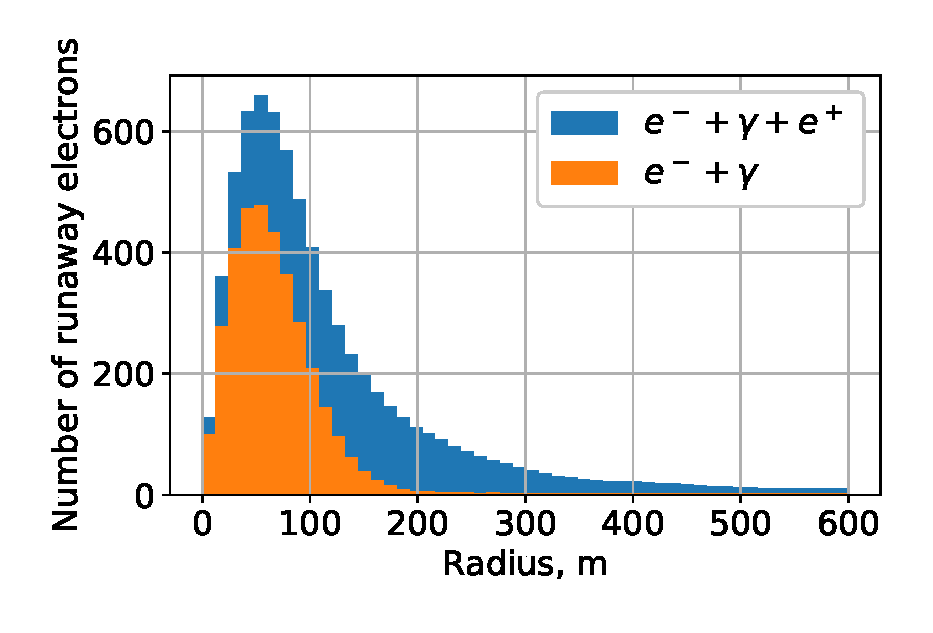
\includegraphics[width=0.45\textwidth]{figures/radial.eps}
    \caption{The distribution of runaway electrons horizontal distance from initial electron creation point for avalanches with length $700$ meters: orange --- without positrons, blue --- with positrons}
    \label{fig:rad}
\end{figure}
%\todo[inline]{How did you normalize the radial distribution? Its strange that there are less electrons in the center of the avalanche}

\section{Conclusions}

In this work we calculated the number of runaway electrons in conditions expected in real thunderclouds (size of the strong field region up to 1200~m and field strength up to 200~kV/m). The simulation itself covers only cell lengths up to 800~m, but it is clear that electron production could be extrapolated. The simulations provides an upper bound for the number of runaway electrons of about $10^6$ runaway electrons or $10^{10}$ total ionizations, which is in accordance with \cite{Gurevich:2001, Dwyer2013_radio} and contradicts to the value presented in \cite{Oreshkin_2018} (more than $10^{16}$ runaway electrons). Especially since Oreshkin’s report considers only electrons, and our results show that introduction of gamma and positron interaction increases the yield of runaway electrons.
Still, even with those interactions, the resulting numbers are by several orders lower than the ones shown in \cite{Oreshkin_2018}. Although the origin of the discrepancy could be investigated further, it is clear that non-relativistic particle dynamics model could not be used to describe generation of enough ionization to produce a lightning discharge.
%

 
%It should be noted that model of Gurevich, Dwyer and Oreshkin is locally, its consider single avalanches in cloud, whereas more difficult model which research interaction of many avalanches (produced due to gamma propagation) in non-uniform field or consider inter-cloud interaction looks promising, because its can generate more runaway electrons and better to ionize cloud.

%In result we can claim that value about $10^{17}$ - $10^{18}$ runaways electrons don't possible in condition specified by Oreshkin's report. For condition which can be observed in nature (length of field area  $<1~km$, field value $<200~kV/m$) single avalanche of runaway electrons contain about $10^4 - 10^6$ runaway electrons.
\acknowledgments
This work is supported by the Russian Science Foundation under grant No. 17-12-01439.


\bibliographystyle{eplbib.bst}
\bibliography{references}
\end{document}   
